\scanpage{27}
% Two manuscript column rules begin alongside the faded first entry.
\noindent\tikz[remember picture,overlay]{
  \coordinate (B27lefttop) at (2.65em,1.2ex);
  \coordinate (B27righttop) at (.955\linewidth,1.2ex);
}

\unsure{302} l.\unsure{15} ``its

303 l.1 ``\deleted{\unsure{with|who}} which will be'' l2 ``we've got'' l.-3 ``image of $A$ by $A$'' - not clear what you mean.

304 l-15 ``commutes with'' also l-13. \deleted{\unsure{l-2} ``play'' \unsure{no|not} ``s}''

305 l.5 ``interpret' l14 ``commutes with''

306 l.19 ``its'' \deleted{l} also l-5. l-4 ``test \uline{category}''

309 l.-8 ``on \uline{the} previous''

312 l-.8 ``isn't'' \deleted{l-6 \unsure{lets|let's}}

313 l9 ``shouldn't'' l.18 ``don't'' l-12 ``commutes with''

\deleted{filtering}\raisebox{1.2ex}[0pt][0pt]{\makebox[0pt][l]{\unsure{\deleted{\unsure{out|at|on|or}}|\unsure{out|at|on|or}}}}\hspace{1.6em}\unsure{l-2|l-7} filtering''

314 l.5 ``isn't'' l.6 ``as is''

315 Sent\tikz[baseline=(B27sentold.base)]{\node[inner sep=0pt] (B27sentold) {\deleted{\unsure{ann|en}}};\node[anchor=base west,inner sep=0pt] at (B27sentold.base west) {en};}ce starting l.7 - difficult to understand. Possibly: 'I add this comment, of course, \deleted{to} in order to ``\uline{push home}'' the point that \uline{no more} with resp... than in any other essential respect. concerning the ability \uline{to express} basic situations.....theory, \uline{does} the cat. ... \uline{stand} singled out. \deleted{(This is \raisebox{1.15ex}[0pt][0pt]{\makebox[0pt][l]{\inserted{certainly}}}true \raisebox{1.15ex}[0pt][0pt]{\makebox[0pt][l]{\inserted{as far as our}}}presumably at the present knowledge goes). \unsure{No|Now}...} (This certainly seems to be so as far as our present knowledge goes)''...

l.17 ``its'' l.-3 'and which \raisebox{1.2ex}[0pt][0pt]{\makebox[0pt][l]{\inserted{would}}}\tikz[baseline=0pt,x=1ex,y=1ex]{\draw[line width=.4pt] (0,-.85)--(.25,-.25)--(.48,-.72);}allow one to compute''

316. l.1 ``shouldn't'' l12 ``$i(a)$ \deleted{it} is a ''\deleted{\unsure{to|is}}

317. l.11 ``its'' l-16 ``isn't''

320 l 8. ``indispensable'' l-15 'developing'' l-8 ``its''

321 l.9 'isn't''

323 l13 ``don't''

326 l-12 \deleted{\unsure{\&|l}}\tikz[baseline=0pt,overlay,x=1em,y=1ex]{\fill (-.4,-.52) circle (.035em);} \& l.-8 \tikz[baseline=(B27comm.base),x=1em,y=1ex]{
  \node[anchor=base west,inner sep=0pt] (B27comm) at (0,0) {``commutes \uline{with}''};
  \node[anchor=base west,inner sep=0pt] at (-.55,2.1) {\inserted{\& l-3}};
  \fill (2.55,3.0) circle (.035em);
  \draw[line width=.4pt] (-.28,.9)--(-.55,-1.9);
  \draw[line width=.4pt] (-.47,-1.1)--(-.35,-1.45)--(-.25,-1.1);
} and

p.327. l7 ``$\alpha:\mathord{\tikz[baseline=0pt,x=1ex,y=1ex]{\draw[line width=.085ex,line cap=round,line join=round] (.19,0)--(.86,1.37)--(1.08,0)--(.71,.025) (.61,.032)--(.19,0) (-.05,.08)--(.51,1.12);}}\longrightarrow \mathord{\tikz[baseline=0pt,x=1ex,y=1ex]{\draw[line width=.085ex,line cap=round,line join=round] (.20,0)--(.83,1.12)--(1.22,.05)--(.82,.04) (.72,.02)--(0,0)--(.64,.99);}}/F$'' should it be '

l-17 ``allows \uline{one} to'' l-16 ``doesn't'' l-14 ``isn't\deleted{\unsure{''}} there!''

l-5 ``don't''

p328 l-12 \deleted{would'nt} should ``wouldn't'' = ``shouldn't''

l-10 doesn't

p329 l.6 $\mathord{\tikz[baseline=0pt,x=1ex,y=1ex]{\draw[line width=.09ex,line cap=round,line join=round] (.16,-.05)--(.77,1.5)--(1.21,.04)--(.16,.0) (.49,1.36)--(-.04,0)--(.21,0);}}$ (doubled side is missing) ``its''

l12 ``don't'' l-13 ``makes sense'' l.-13 ``semisimplicial. \tikz[baseline=0pt,x=1ex,y=1ex]{\draw (0,-.6)--(.45,1.7); \draw (.14,.1)--(.43,-.1);}\tikz[baseline=0pt,overlay,x=1em,y=1ex]{\fill (1.0,5.3) circle (.035em);\fill (.84,4.9) circle (.035em);}\raisebox{1.7ex}[0pt][0pt]{\inserted{l-5 ``enveloping\unsure{''|'}}} \margin{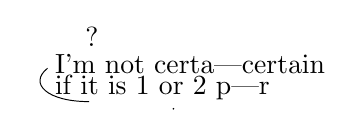
\begin{tikzpicture}[x=1em,y=1ex]
  \node[anchor=west,inner sep=0pt] at (1.1,2.2) {?};
  \node[anchor=west,inner sep=0pt] at (0,0) {I'm not \unsure{certa|certain}};
  \node[anchor=west,inner sep=0pt] at (0,-2.0) {if it is 1 or 2 \unsure{p|r}};
  \draw[line width=.35pt] (-.25,-.4) .. controls (-.95,-1.7) and (-.25,-3.2) .. (1.25,-3.2);
  \fill (4.3,-3.8) circle (.035em);
\end{tikzpicture}}
% slanted; right edge of the note is clipped

p.333 l.-12 ``makes sense''

p.334 l.3 '$b\in A_{n-1}$'' l-6 ``its'' also in l-5.

% The same two rules continue to the foot, beyond the final correction entry.
\noindent\tikz[remember picture,overlay]{
  \coordinate (B27foot) at (0,-1.2ex);
  \draw[line width=.35pt] (B27lefttop) -- (B27lefttop |- B27foot);
  \draw[line width=.35pt] (B27righttop) -- (B27righttop |- B27foot);
}

% archive sheet number: 26
